\subsection{Shadow DOM}
\label{sec:3_WC_Shadow_DOM}

Das folgende Kapitel basiert ausschließlich auf der Spezifikation von Shadow-DOM des W3C \citereset \autocite[siehe][]{GlazkovShadowDOM.2013} und auf dem Artikel \glqq Shadow DOM 101\grqq\ \citereset \autocite[siehe][]{Cooney.2013}.

Mit Hilfe von Shadow-DOM können Elemente mit einer neuen Art von Knoten verbunden werden. Diese neue Art von Knoten wird auch \glqq Shadow-Root\grqq\ genannt. Ein Element, dass einer Shadow-Root zugeordnet ist, wird auch \glqq Shadow-Host\grqq\ bezeichnet. Anstatt den Inhalt eines Shadow-Hosts zu rendern, wird immer der des Shadow-Roots gerendert.

\begin{lstlisting}[language=HTML, caption={[Shadow-Root Beispiel eines Buttons \citereset \autocite{Cooney.2013}] Shadow-Root Beispiel eines Buttons}, label={lst:3_ShadowDomBasic1}, escapeinside={@}{@}]
<button>Hello, world!</button>
<script>
  var host = document.querySelector('button');
  var root = host.createShadowRoot();
  root.textContent = 'Hello, shadow DOM!';
</script>
\end{lstlisting}

Code-Beispiel \ref{lst:3_ShadowDomBasic1} rendert zuerst das in Abbildung \ref{sfig:3_ShadowDom1} auf Seite \pageref{sfig:3_ShadowDom1} gezeigte Ergebnis. Danach wird mit Hilfe von JavaScript und Shadow-DOM das Element, wie in Abbildung \ref{sfig:3_ShadowDom2} auf Seite \pageref{sfig:3_ShadowDom2} zu sehen ist, verändert.

\begin{figure}[h]
  \centering
  \subfloat[HTML gerendertes Element]{
    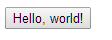
\includegraphics[]{images/SS2.png}
    \label{sfig:3_ShadowDom1}
  }
  \qquad
  \subfloat[HTML Element mit Hilfe von JavaScript und Shadow DOM manipuliert]{
    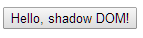
\includegraphics[]{images/SS1.png}
    \label{sfig:3_ShadowDom2}
  }
  \caption[
    Beispiel einer Shadow-Root Node
  ]{
    Beispiel einer Shadow-Root Node
  }
  \label{sfig:3_ShadowDom}
\end{figure}

Wenn das \lstinline|<button>|-Element nach seinem Inhalt mittels der \lstinline|textContent|-Eigenschaft abgefragt wird, wird das Resultat nicht \lstinline|"Hello, shadow DOM!| zurückgeben, sondern \lstinline|"Hello, world!"|, da die DOM-Unterstruktur unter der Shadow-Root vollständig gekapselt ist.

Es ist zu erwähnen, dass dies ein sehr schlechtes Beispiel für Suchmaschinen, Browser-Extension, Screen-Readers etc. ist, da sämtlicher Inhalt des Shadow-DOMs nicht für diese erreichbar ist. Shadow-DOM ist nur für sematisch bedeutungsloses Markup, das benötigt wird um eine Webkomponente zu erstellen, gedacht.

\subsubsection{Trennung von Inhalt und Darstellung}
\label{sec:3_WC_Shadow_DOM1}

Code-Beispiel \ref{lst:3_ShadowDomBasic2} auf Seite \pageref{lst:3_ShadowDomBasic2} wird als Ausgangsbasis dieses Beispiels genommen \citereset \autocite[siehe][]{Cooney.2013}. Abbildung \ref{fig:3_ShadowDom2} auf Seite \pageref{fig:3_ShadowDom2} zeigt diese Grundbasis, um mit darauffolgenden Schritten sämtlichen Inhalt von der Darstellung zu trennen. Dies garantiert, dass der tatsächliche Inhalt für Suchmaschinen, Screen-Readers, Browser-Extensions etc. erreichbar und die Darstellung für die Endbenutzerin beziehungsweise den Endbenutzer \glqq unsichtbar\grqq\ ist.

\begin{lstlisting}[language=HTML, caption={Namensschild ohne Shadow-DOM - Ausgangsbasis um Inhalt von Darstellung zu trennen}, label={lst:3_ShadowDomBasic2}, escapeinside={@}{@}]
<style>
.outer {
  border: 2px solid brown;
  border-radius: 1em;
  background: red;
  font-size: 20pt;
  width: 12em;
  height: 7em;
  text-align: center;
}
.boilerplate {
  color: white;
  font-family: sans-serif;
  padding: 0.5em;
}
.name {
  color: black;
  background: white;
  font-family: "Marker Felt", cursive;
  font-size: 45pt;
  padding-top: 0.2em;
}
</style>
<div class="outer">
  <div class="boilerplate">
    Hi! My name is
  </div>
  <div class="name">
    Bob
  </div>
</div>
\end{lstlisting}

\begin{figure}[h]
\centering
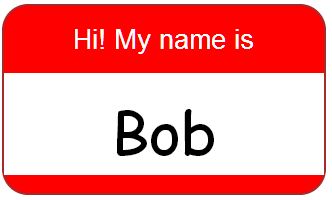
\includegraphics[height=5.0cm]{images/SS3.png}
\caption[
  Ausgangsbeispiel von der Trennung von Darstellung und Inhalt bei Shadow-DOM \citereset \autocite{Cooney.2013}
]{Ausgangsbeispiel von der Trennung von Darstellung und Inhalt bei Shadow-DOM}
\label{fig:3_ShadowDom2}
\end{figure}

Dadurch, dass dem DOM-Tree Kapselung fehlt, ist die gesamte Struktur des Namensschildes im Dokument sichtbar. Wenn beispielsweise externe Elemente auf der Webseite dieselben Klassennamen verwenden, würden diverse CSS-Klassen überschrieben werden.

\begin{enumerate}
\litem{Verstecken von Darstellungsdetails} \hfill \\
Semantisch gibt es nur zwei wichtige Informationen bei diesem Beispiel:
\begin{enumerate}
\item Es ist ein Namensschild
\item Der Name ist \glqq Bob\grqq .
\end{enumerate}
Daraus wird das Markup erstellt, das semantisch näher bei der gewünschten Information ist (siehe Code-Beispiel \ref{lst:3_ShadowDomBasic3}).

\begin{lstlisting}[language=HTML, caption={[Darstellung des Markups mit der gewünschten Information ohne Darstellung \citereset \autocite{Cooney.2013}] Darstellung des Markups mit der gewünschten Information ohne Darstellung}, label={lst:3_ShadowDomBasic3}, escapeinside={@}{@}]
<div id="nameTag">Bob</div>
\end{lstlisting}

Des Weiteren wird sämtlicher Code, der der Darstellung dient, in ein \lstinline|<template>|-Element gepackt (siehe Code-Beispiel \ref{lst:3_ShadowDomBasic4}). Dies ist notwendig um sämtliche Darstellungsdetails von dem eigentlichen Inhalt trennen zu können.

\begin{lstlisting}[language=HTML, caption={[Darstellung des Markups mit der gewünschten Information mit Hilfe von einem Template \citereset \autocite{Cooney.2013}] Darstellung des Markups mit der gewünschten Information mit Hilfe von einem Template}, label={lst:3_ShadowDomBasic4}, escapeinside={@}{@}]
<div id="nameTag">Bob</div>
<template id="nameTagTemplate">
  <style>
    .outer {
      border: 2px solid brown;
      border-radius: 1em;
      background: red;
      font-size: 20pt;
      width: 12em;
      height: 7em;
      text-align: center;
    }
    .boilerplate {
      color: white;
      font-family: sans-serif;
      padding: 0.5em;
    }
    .name {
      color: black;
      background: white;
      font-family: "Marker Felt", cursive;
      font-size: 45pt;
      padding-top: 0.2em;
    }
  </style>
  <div class="outer">
    <div class="boilerplate">
      Hi! My name is
    </div>
    <div class="name">
      Bob
    </div>
  </div>
</template>
\end{lstlisting}

Zu diesem Zeitpunkt wird \glqq Bob\grqq\ das einzige sein, das gerendert wird. Das Template enthält sämtlichen Code der Darstellung und muss nun beispielsweise mit JavaScript hinzugefügt werden. In Code-Beispiel \ref{lst:3_ShadowDomBasic5} auf Seite \pageref{lst:3_ShadowDomBasic5} wird zuerst eine Shadow-Root am Element \lstinline|<div id=nameTag></div>| erstellt. Danach wird nach dem Template gesucht und der Inhalt dieses Templates an die Shadow-Root angefügt.

\begin{lstlisting}[language=JavaScript, caption={[Hinzufügen des Inhalts eines Templates in eine Shadow-Root \citereset \autocite{Cooney.2013}] Hinzufügen des Inhalts eines Templates in eine Shadow-Root}, label={lst:3_ShadowDomBasic5}, escapeinside={@}{@}]
<script>
  var shadow = document.querySelector('#nameTag').createShadowRoot();
  var template = document.querySelector('#nameTagTemplate');
  shadow.appendChild(template.content);
</script>
\end{lstlisting}

Da nun eine Shadow-Root mit Markup vorhanden ist, wird das Namensschild wieder korrekt angezeigt. Wenn das Element mit Hilfe der Entwickler-Tools im Browser inspiziert wird, wird nur die gewünschte Information ohne Darstellungselemente angezeigt. Dies zeigt, dass durch die Verwendung von Shadow-DOM sämtliche Darstellungendetails im Shadow-DOM gekapselt wurden und von außen nicht erreichbar sind.

\litem{Trennung von Inhalt und Darstellung} \hfill \\
Mit Hilfe von Code-Beispiel \ref{lst:3_ShadowDomBasic4} und \ref{lst:3_ShadowDomBasic5} werden sämtliche Darstellungsdetails versteckt, jedoch wurde der Inhalt noch nicht mit der Darstellung getrennt. Wenn beispielsweise der Name des Namensschildes ausgetauscht werden müsste, müsste dies an zwei Stellen gemacht werden: Einerseits an der Stelle im Template und andererseits an der Stelle des \lstinline|<div id=nameTag></div>|-Elements.

Um den tatsächlichen Inhalt von sämtlichen Darstellungen zu trennen, muss eine Komposition von Elementen benutzt werden. Das Namensschild setzt sich einerseits aus dem roten Hintergrund mit den \glqq Hi! My name is\grqq -Text zusammen und andererseits aus dem Namen der Person.

Als Programmiererin beziehungsweise Programmierer einer Komponente kann entschieden werden, wie die Komposition des erstellten Elements funktionieren soll. Mit Hilfe des \lstinline|<content>|-Elements können Kompositionen erstellt werden. Dieses Element erstellt einen \glqq Insertion-Point\grqq\ in der Darstellung und sucht Inhalte aus dem Shadow-Host, die an dieser Stelle angezeigt werden sollten.

\begin{lstlisting}[language=HTML, caption={[Erweiterung des Code-Beispiels \ref{lst:3_ShadowDomBasic4} mit dem <content>-Element \citereset \autocite{Cooney.2013}] Erweiterung des Code-Beispiels \ref{lst:3_ShadowDomBasic4} mit dem <content>-Element}, label={lst:3_ShadowDomBasic6}, escapeinside={@}{@}]
<div id="nameTag">Bob</div>
<template id="nameTagTemplate">
  <style>
    .outer {
      border: 2px solid brown;
      border-radius: 1em;
      background: red;
      font-size: 20pt;
      width: 12em;
      height: 7em;
      text-align: center;
    }
    .boilerplate {
      color: white;
      font-family: sans-serif;
      padding: 0.5em;
    }
    .name {
      color: black;
      background: white;
      font-family: "Marker Felt", cursive;
      font-size: 45pt;
      padding-top: 0.2em;
    }
  </style>
  <div class="outer">
    <div class="boilerplate">
      Hi! My name is
    </div>
    <div class="name">
      <content></content>
    </div>
  </div>
</template>
\end{lstlisting}

In Code-Beispiel \ref{lst:3_ShadowDomBasic6} auf Seite \pageref{lst:3_ShadowDomBasic6} wird das Namensschild mit dem vom Shadow-Host projizierten Inhalt in das \lstinline|<content>|-Element gerendert. Dies vereinfacht die Struktur des Dokuments, da der Name nur noch an einer Stelle vorhanden ist. Müsste nun der Name aktualisiert werden, wäre das mit folgender Methode möglich: \lstinline|document.querySelector('#nameTag').textContent = 'Shellie';|.

Das Namensschild wird automatisch nach Zuweisung eines neuen Namens aktualisiert, da der Inhalt vom Namensschild in das \lstinline|<content>|-Element projiziert wird. Somit wurde die Trennung von Inhalt und Darstellung erreicht.
\end{enumerate}